\documentclass[../_main/handlingar.tex]{subfiles}

\begin{document}
\proposition{Budgetjustering för källarmästeriet och sexmästeriet }

    Källarmästeriet har under flera år presterat under den budget som satts för utskottet samtidigt som sexmästeriet snarare haft problem att inte gå för mycket över budget. Det är dessutom så att Källarmästeriet belastas med den kostnad som uppstår för differenser i alkohollagret och sektionens stadigvarande tillstånd, två saker som nyttjas av Sexmästeriet. Att erbjuda mat och dryck till konkurrenskraftiga priser är källarmästeriets främsta mål och jag ser därför att det är eftersträvansvärt att inte behöva höja priserna för att klara budgeten. Enligt gjorda kalkyler är detta möjligt men utrymmet för oförutsedda händelser och utsvängningar under året är synnerligen begränsat. Utökad budget skulle ge ökad möjlighet till flera saker, exempelvis att även kunna hålla gillen på dagar utöver de dagar då vi har stadigvarande tillstånd, för samarbeten med andra utskott, anpassning till påsk och andra helger och liknande. Vi skulle även få mer möjlighet att hålla roliga och temaenliga gillen med pynt och drinkar, vilket jag anser kommer sektionen till nytta. Dessutom går delar av källarmästeriets budget till funktionärsvård genom att jobbare förses med mat och godis då de jobbar. Detta är viktigt och inget som bör övervägas att begränsas för att hålla en snäv budget. 

Sexmästeriet har som ovan nämnt haft problem med att inte gå med för mycket vinst de senaste åren. Detta kommer antagligen av många evenemang med alkoholservering där vi enligt lag behöver gå med vinst. Att sexmästeriet har ett lågt vinstkrav motiveras av att det kommer sektionens funktionärer till nytta genom att det blir billigt att gå på sittning. Det kan det fortsatt vara med en i sammanhanget liten ökning i vinstkrav. Det kommer även i högsta grad sektionens funktionärer till nytta att det är fortsatt billigt med mat och dryck i Edekvata samt att det ges möjlighet till fler gillen och god vård av utskottets funktionärer.  

Genom en omfördelning mellan Sexmästeriets och Källarmästeriets budgetar så påverkas inte årsbudgeten men de två utskotten kommer få budgetar som svarar mer mot det som utskotten naturligt presterar. Se nedan sammanställning av de senaste årens budget och resultat för de båda utskotten.


    \begin{center}
        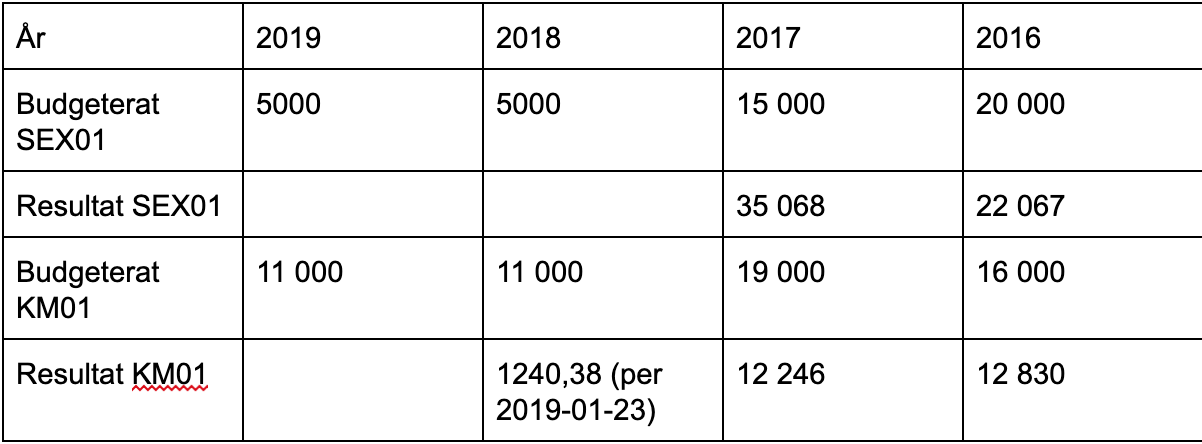
\includegraphics[scale=0.5]{../_res/budget_resultat.jpg}
    \end{center}


Styrelsen yrkar därför 
\begin{attsatser}
    \att sänka budgetposten Gille under KM01 med 5000 kr till 6 000 kr.
    \att höja budgetposten E6 allmänt under SEX01 med 5000 kr till 10 000 kr. 
\end{attsatser}

\begin{signatures}{1}
    \ist
    \signature{\krog}{Davida Åström}
\end{signatures}

\end{document}
